\documentclass[a4paper]{article}

\usepackage{sectsty}
\usepackage{graphicx}
\usepackage{listings}
\usepackage{subcaption}
\usepackage{framed}
\usepackage{hyperref}
\sectionfont{\fontsize{12}{15}\selectfont}
\usepackage[left=90.00pt, right=90.00pt, top=100.00pt, bottom=100.00pt]{geometry}
\title{Homework Assigment 4: Modelling pandemics \\ \large Scientific Software / Technisch Wetenschappelijke Software 2020}
\author{If I do not change this, the person grading my report will not know who I am!\\ It could be a good idea to change this before writing my report.}

\lstset{
	language=c++,
	%    basicstyle={\ttfamily \small},
	basicstyle={\ttfamily \small},
	%    keywordstyle=\underline,
	numberstyle={\footnotesize},
	%    morekeywords={ones,mod,isprime,inline,unique,factor,@},
	%    flexiblecolumns=false,
	%    emph={gamma,beta},
	%    emphstyle=,
	columns=fullflexible,
	%    columns=flexible,
	%    commentstyle={\slshape},
	%    commentstyle={\normalfont},
	commentstyle={\ttfamily},
	stringstyle={\ttfamily \bfseries},
	showstringspaces=false,
	%    indent=1em,
	%    xleftmargin=0.5em,
	breaklines=false,
	%    frame={l},
	captionpos={t},
	upquote=true, % such that we can copy-paste the code...
	%    mathescape=true,
	%    frame=single,     % boxed in a single line
	%    frame=L,          % double line on the left
	%    frame=l,          % single line on the left
}
\newcommand{\answer}[1]{\vspace{-0.75em}\begin{framed} #1 \end{framed}\vspace{-0.75em}}
\begin{document}

\maketitle
\section*{Practical information}
\begin{itemize}
	\item Number of hours spent: 30
\end{itemize}


\section*{General}
\begin{enumerate}
	\item Which concepts from the lectures and exercise sessions did you use? Where? Which concepts didn't you use? Why not?
	\answer{
		
	\begin{itemize}
		\item assertions, debugging levels - using \#ifdef statements to add additional (or supress completetly) debugging info using compiler flags
		\item templates and concepts - for ODE solver to handle different ODE system and use all the methods to solve said systems, also the ODE system objects are templated with working precission and size type, which than propagates to all the other class/functions
		\item templates and concepts - for the optimization algorithms so that they can take any target functor which satisfies the necessary concept
		\item functions as arguments (functors) and scratch arrays - for example line search or even the ODE solving methods are kind of functors - this should save time on repeated calls, because "working space" (vectors, matricies) are only allocated on the creation of such functor
		\item type traits - only to check on creation of ODE equations system if size is integral and value is a float - I could probably do that in every class/function to make the code even safer
		\item information hiding - in classes for solvers, methods and LSE evaluation
		\item algorithm abstraction - ODE solver as well as optimization algorithms CGM and BFGS (haven't tested for the latter though)
		\item constants known at compile time - mainly dimension of ODE equations system but also the number of optimized parameters in CGM and BFGS is known at compile time.
	
	\end{itemize}
}
	\item Are there changes or improvements you wanted to make but where unable to implement due to lack of time?
	\answer{
	I guess the code could still get a bit safer with more asserts and especialy type traits asserts in various templates - checking if numbers is actually floating or integral type.
	
	I would also like to comment the code a bit more - adding concept assuptions for equations, solvers, functors and even matricies and vectors.
	
	Some general settings file, which would contain all the different meta paremeters that are now scattered across the appropriate classes which use them.
	
	Safer reading of parameters and observations from file.
}
	\item Are there other general comments you want to make?
	\answer{
	It can seem a bit unfortunate that when tempalting a method, it has to recieve ODE system as template argument, so we cannot reuse the same method object for some other ODE system (with reallocating ). But I wanted to keep the safe behaviour of this approach. This is however easily changable by making \texttt{dim} a non-static variable and adding a \texttt{resize()} method to change the dimension the solver assumes to have (reallocating all scratch space needed).
	
	Accross the different programs, different SIQRD parameters files are used to make my life easier. The simulation1.exe still uses the original \texttt{parameters.in}.
	
	The vector of SIQRD parameters is in alphabetic order \texttt{alpha, beta, gamma, delta, mu}, because the order in which they appear in parameters.in is hard to remember.
}
\end{enumerate}
\section*{Part 1: Simulating the pandemic}
\begin{enumerate}
	\item Have you made any modification to the structure/organization of your ordinairy differential solvers based on earlier feedback?
	\answer{
	I restructered the code to pre-allocate memory for ODE solving methods at construction-time, so that this does not need to be done inside any loop.
}
	\item \textbf{Compare your Fortran code and your C++ code.} How does your C++ implementation differ from your Fortran implementation? What C++ specific features did you use? Are there features that you could use in Fortran but that are not available in C++? Are there design decisions that you have to take into account when working with C++ that you do not have to make (can not make) in Fortran? Was it easier to implement the functionality in Fortran or in C++?
	\answer{
	My Fortran implementation was very problem specific. In C++ I tried to make everything as general as possible, so now the solvers are decoupled from SIQRD application. I tried to do that before in Fortran but had problems beacuse of different interfaces of forward and backward methods. This kind of polymorfism was much easier to accomplish in C++. I tried to use OOP features that C++ offers to acomplish new features and make my life easier while programming it. The basic functionality was definitely easier to implement in Fortran. Probably because we had multiple exercise sessions on the basics of matrix and vectors operations. These things are not so comfortable to work with in C++ as they are in Fortran. I really liked Fortran, because it took a lot less time to get a basic working example of the simulation algorithm. On the other hand in C++ is easier to make algorthms/functions more abstract, as I already mentioned. 
}
	\item Your simulation code must now accept more general ordinary differential equations. Which C++ features did you need to use to achieve this extra flexibility? How would you do this in Fortran 90/95?
	\answer{
		For any specific ODE, there has to be a new class which satisfies necessary concept - \texttt{OdeSystem}, meaning that is has some dimension, operator to evaluate the derivates, also a function to compute jacobian (for backward Euler) and a function to provide vector of initial conditions. 
		
		In Fortran I would probably have to pass these functions separately as arguments to ODE solver subroutine, which would result in a large number of arguments. 
		
		Also making use of scratch space in ODE dolver methods would be a bit more chalanging, I would probably have to ask the method the necessary size of the scratch space for example like the eigenvalues solving (DGESV I think it was) routine of LAPACK does.
	
}
	\item In sumulation2.cpp it is asked how can you pass the differential equation to your ODE solver code? Discuss all possibilities.
	\answer{
	The basic approach would be passing function pointer(s), which would probably be a similar code structure as in Fortran. This wasy, the code could than accept an actual funciton pointer or a lambda expression. It was already mentioned that I opted for an approach using a functor class which encapsulates all this and exposes only necessary members, plus can have other functionality like computing the jacobian and initial condition manipulation. It is not passed to solver as a dynamicaly interpreted functor but using a template.
}
	\item How did you avoid using an explict for loop?
	\answer{
		Using and \texttt{std} algorithm and a lambda expression like shown on the code snippet below.
	}

\begin{lstlisting}
int i = 0;
auto fun = [&i]() { return ++i * 0.01; };
std::generate(ret.begin(), ret.end(), fun);
\end{lstlisting}

	\item Are there other design decisions you want to mention?
	\answer{}
\end{enumerate}
\subsection*{Verify your code for the SIQRD model}
% Also include your figures seperately in your ZIP.

\begin{figure}[!h]
	\centering
	\begin{subfigure}{0.32\linewidth}
		\centering
		\includegraphics[width=\textwidth]{figs/fwe_no_measures}
	\end{subfigure}
	\begin{subfigure}{0.32\linewidth}
		\centering
		\includegraphics[width=\textwidth]{figs/bwe_quarantine}
	\end{subfigure}
	\begin{subfigure}{0.32\linewidth}
		\centering
		\includegraphics[width=\textwidth]{figs/heun_lockdown}
	\end{subfigure}
\caption{Figures as in first assignment.}

\end{figure}
\begin{figure}[!h]
	\centering
	\includegraphics[width=\textwidth]{figs/jc_miller}
	\caption{parameters for this calculation are
		$\label{eq:parameters2ndExample}
		\beta = 10;\,\,
		\gamma = 1;\,\,
		\mu=\,\alpha=\,\delta = 0;\,\,
		S_0 = 0.95;\,\,
		I_0 = 0.05.\,\,
		$}
\end{figure}
\begin{figure}[!h]
	\centering
	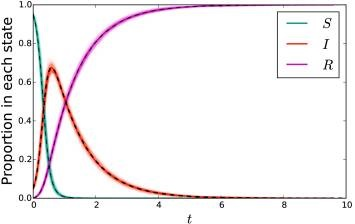
\includegraphics[width=0.3\textwidth]{figs/sirMiller.jpg}
	\caption{from article  \href{https://www.ncbi.nlm.nih.gov/pmc/articles/PMC5963332/}{Mathematical models of SIR disease spread with combined non-sexual and sexual transmission routes}}
\end{figure}
\subsection*{Verify your code for the general ODE}
	\answer{Verification is done by comparing the results to analytical solution at the latest time of the calculation. I relative error is printed to console when running \texttt{simulation2.exe} and looks as follows: }
\begin{lstlisting}
fwe: Relative error at time 500: 0.00330854

bwe: Relative error at time 500: 2.64313e-07

heun: Relative error at time 500: 1.8886e-08 
\end{lstlisting} 

\section*{Part 2: Parameter estimation from observations}
\begin{enumerate}
	\item \textbf{How did you optimize the performance (execution time and memory usage) of the parameter estimator code?} What part of the code has the most influence on the execution time? What tools did you use to assess the performance of your code? How did you avoid unessecary memory usage or copies? After having an initial working version, did you make changes to improve performance? 
	\answer{
\begin{itemize}
	\item using scratch space to avoid allocating vectors and matricies over and over again
	\item same for variables inside loops, i try to declare them/ allocate outside
	\item using \texttt{ublas} routines to compute norms 
	\item using \texttt{.assign()} to avoid unnecessary copzing as well as \texttt{noalias(A)}
	\item I used valgrind to check if possible imporvements have actually worked.
	\item i tried using gprof but could not make much sense out of it, because it was dominated by ublas calls.
	\item in my initial version I didn't pay much attention to memory efficiency or number allocations. I started correcting and improving performance after I was more or less sure of the corectness
	\item I also restructured some parts of the code in order to decouple the optimization algorithms from siqrd implementation
\end{itemize}	
}
	\item \textbf{Flexibility.} How did you achieve flexibility in your code? How do you switch between the solvers for the ordinary differential equation? 
	\answer{
	Mostly using templates. ODE solving methods are passed as template argument to OdeSolver class, which then uses them to solve the system.
}
	\item \textbf{Verification.} How did you verify your code? Are there other checks you preformed?
	\answer{
	Mainly by plotting the observations against results of simulations, which were run with the parameters from CGM and BFGS. I also generated a few observations myself (using the simulation) and ran the optimizations on them as well. Also the starting parameters were varied to validate the robustness of the implementation. I found that the algorithms work even for quite bad assumptions but there are limits to that as well.
}
	\item How do you update the parameters of your SIQRD model?
	\answer{
	The aplication specific class \texttt{LSE\_siqrd} passes a vector of parameters to SIQRD equations object to update the parameters. Same way is used to pass new initial conditions, that are read from \texttt{observations} file.
}

\end{enumerate}
\subsection*{Verify your code}
\begin{figure}[!h]
	\centering
	\begin{subfigure}{0.49\linewidth}
		\centering
		\includegraphics[width=\textwidth]{figs/bwe_bfgs1}
	\end{subfigure}
	\begin{subfigure}{0.49\linewidth}
		\centering
		\includegraphics[width=\textwidth]{figs/heun_cgm2}
	\end{subfigure}
\caption{Results of simulation done on observations one and two. Observed quantities are plotted only by \textbf{x} mark, ode simulation by solid line.}
\end{figure}
\begin{itemize}
	\item Does the parameter estimator work for the different ODE solvers? Do the obtained parameters differ?
	\answer{
		Yes the implementation works with all solvers. With Euler backward, sometimes in the first LSE evaluation, the convergenece criteria of Newton's method are not met. This however does not impact the final solution - the CGM and BFGS converge in same (or sometimes even less) iterations as when using Euler forward method.
		
		The final values differ across the methods but mostly in magnitute of a few percent. This was expected since the methods have always "disagreed" on the final results unless the time step is very small. 
	}
\end{itemize}
\section*{Extra questions}
\begin{enumerate}
	\item What C++-features did you use to achieve this?
	\answer{
	If I would do it, I would make use of template specialization for Euler backward method and then instead of computing the inversion, handle each row (= equation) separately.	
}
	\item Did you make other improvements? How big is their effect on the execution time, the number of calls to the ODE solver or the memory usage?
	\answer{
	In LSE functor I save the population size in constructor call, instead of getting it from the equations every \texttt{LSE\_siqrd()} call. This actually saved additional 10\% of time (timed with optimization flags).
}
	\item Are there other design decision you want to mention?
	\answer{}
\end{enumerate}

\end{document}